
\documentclass[journal]{IEEEtran}

%%%%%%%%%%%%%%%%%%%%%%%%%%%%%%%%%

%Linguagem e acentuação\textsl{}
\usepackage[utf8]{inputenc}
\usepackage[T1]{fontenc}
\usepackage{lmodern}

%Imagens
\usepackage{graphicx}

%Tabelas
\usepackage{multicol}
\usepackage{booktabs}
\usepackage{multirow}

%Algoritmo
\usepackage[english, ruled, lined, linesnumbered]{algorithm2e}


%Gramática
\usepackage[nounderscore]{syntax}
\usepackage{amsmath}
\grammarindent 80pt

%Renomear TABLE para TABELA
%\renewcommand{\tablename}{TABELA.}
%\renewcommand{\refname}{Referências}
%%%%%%%%%%%%%%%%%%%%%%%%%%%%%%%%%

% correct bad hyphenation here
\hyphenation{cons-ta-tar}


\begin{document}
%
% paper title
% can use linebreaks \\ within to get better formatting as desired

\title{A grammatical evolution approach to generate clustering algorithms}


\author{
	Ricardo Henrique Remes de Lima,
	Vidal Daniel da Fontoura}

% The paper headers
%\markboth{Journal of \LaTeX\ Class Files,~Vol.~6, No.~1, January~2007}%
%{Shell \MakeLowercase{\textit{et al.}}: Bare Demo of IEEEtran.cls for Journals}

% make the title area
\maketitle

\begin{abstract}

Resumo

\end{abstract}

\begin{IEEEkeywords}
	Clustering, Grammatical Evolution, Genetic Programming, Hyper-Heuristic.
\end{IEEEkeywords}

\IEEEpeerreviewmaketitle

\section{Introduction}

More data has been gathered because of the modern methods of data collection. The demand for grouping and filtering important data and collect useful information is increased. Clustering is the unsupervised classification of patterns (observations, data items, or feature vectors) into groups (clusters). Clustering approaches applications has increased in various areas of Artificial Intelligence, data mining, image recognition, data statistics, etc. The main goal is to determine the intrinsic grouping in a set of unlabeled data \cite{ahalya2015data}.

The main problem in the application of clustering algorithms, is that, an algorithm can have a good performance in a certain type of problem or test instances, and have a poor performance in other problem or test instances of the same problem. Although some researchers have suggested that "the objective of cluster analysis is simply to find a convenient and valid organization of the data, not to establish rules for separating future data into categories" \cite{jain1988algorithms}, it is often desired to use the resulting clustering to predict the labels of unseen data.

Many real world optimization problems are complex and very difficult to solve. This is due to the large, and often heavily constrained, search spaces, which make their modeling a very complex task. Heuristic methods are usually used in this cases, when the optimal solution is hard to find in a reasonable amount of time. The main aim of the heuristic is to find a good solution within a realistic amount of time \cite{sabar2013grammatical}. Meta-heuristics

Genetic Programming (GP) is a type of Evolutionary Algorithm (EA) that has been studied more over the years. GP is a domain-independent method that genetically breeds a population of computer programs to solve a problem, it evolves the solutions by the application of selection, mutation and crossover operators \cite{poli2014genetic}. The difference from Evolutionary Algorithms, is that GP is used to evolve computer programs, and has its individuals represented by syntax trees.

Deeper in the idea of evolving computer programs, one of the used approaches in Genetic Programming, is the Grammatical Evolution, where a BNF (Backus-Naur Form) grammar is used to generate sentences for a given language, this sentences are mapped into the computer programs that are evaluated by the algorithm. Finally the generated algorithm is executed and its performance is used as feedback for the evolving process.

Based of the topics presented above, this paper tests if is possible to apply the Grammatical Evolution approach for the Clustering problem in order to generate a good and generic algorithm for data classification. If the algorithm generated can get fair results when applied to different instances of different problems.

To test if generated algorithms provided by the Grammatical Evolution have a good performance over the different problem and test instances, they were compared to other well-known technique for data classification, the \textit{k-means} algorithm.


\section{Theoretical Foundation}

This section is about some of the important subjects mentioned in this paper.

\subsection{Genetic Programming}

Genetic Programming (GP) is a systematic method for getting computers to automatically solve a problem from a high-level statement of what need to be done \cite{koza2005genetic}. Having a similar behavior to the Genetic Algorithms (GAs), the GP iteratively evolves a population of computer programs, applying the selection, crossover and mutation operators, to try to improve their fitness, and increase the chances of a individual being part of future generations.

Different from the AG, the GP works with computer programs, and because of this, the use of a different structure for the individual's representation of the population is necessary. There are many approaches for representing individuals, some of the most used are: the syntax tree and grammatical evolution.

The original formulation of genetic programming was done with a tree representation. Here, each node on the tree is a function which takes its children as inputs and sends its output to its parent. Each subtree is a complete sub-program. However, there is no capacity for parts of the tree to be reused in a calculation, which make some things more difficult \cite{harris2015comparison}.

Grammatical genetic programming uses a genotype that, rather than directly representing a set of nodes, represents a numbered list of grammatical expansions which eventually produce its nodes. This potentially allows for a lot more control by the user over the search space, and also facilitates the use of multiple data types in the algorithm. The genotype is represented linearly but can be decoded into a tree for execution and evaluation. In terms of what can be represented, unless restricted in its grammar this GP variant has the same search space as with tree GP \cite{harris2015comparison}.

\subsubsection{Genetic Programming Nodes}

In Genetic programming, every variant of algorithm uses the same set of algorithm nodes. The nodes can take parameters as inputs or not, and produce an output. Each node is considered an independent algorithm, and can be evaluated separated.

The nodes can be divided in two main groups: terminal nodes and non-terminal nodes. Terminal nodes are nodes that take no inputs, and are usually values ou variables used as inputs. Non-terminal nodes are nodes that take inputs and use them to produce the output, the inputs are usually terminal nodes or the output of other non-terminal node.

\subsection{Grammatical Evolution}

Grammatical evolution is a grammar based form of genetic programming. GE accomplishes the mapping process by combining a context free grammar (CFG) with a rule selection mechanism implemented using a genetic algorithm \cite{byrne2015optimising}.

The main difference between GE and GP, is that in GP, both genotype and phenotype of the individual that undergoes evolution is a derivation tree, while in GE, genotype and phenotype have different encoding structures. The genotype is represented as a linear string of codons (sequence of 8 bits) of variable size, which is then decoded into a vector of integers. The phenotype, which is the structure that defines fitness, is represented by a derivation tree (resulting from the application of a grammar) \cite{cerri2013grammatical}. The clear distinction between the genotype and phenotype in GE allows the evolutionary process to be performed on the search space (variable length linear genotypic) without needing to tailor the diversity-generating operator to the nature of the phenotype \cite{sabar2013grammatical}.

The grammar is a set of structural rules that define the composition of sentences for a given language. Grammatical rules provide a concise way of restricting a language while allowing endless variation through recursive application of the rules\cite{byrne2015optimising}. The grammar is represented by Backus-Naur Form (BNF). The program is generated by using a integer vector, where each códon (vector position) value, is used to determine which production rule in the BNF grammar will be used.

\begin{figure}[!htb]
	\centering
	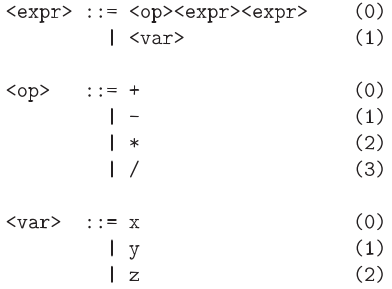
\includegraphics[scale=.8]{figures/grammar.png}
	\caption{Example fo basic grammar. \cite{ryan1998grammatical}}
	\label{fig:grammar}
\end{figure}

The Figure \ref{fig:grammar} shows a basic BNF (Backus-Naur Form) grammar, that can be used to generate simple math equations. In the group of terminal nodes, we have: +, -, *, /, as operations and x, y and z as variables. For the non-terminal nodes, we have: $<$op$>$, $<$expr$>$ and $<$var$>$.

\begin{figure}[!htb]
	\centering
	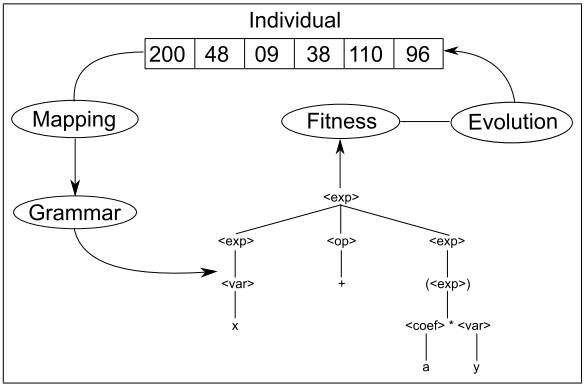
\includegraphics[scale=.6]{figures/ge_algo.png}
	\caption{Basic scheme for mapping process. \cite{cerri2013grammatical}}
	\label{fig:ge_algo}
\end{figure}

A mapping process is needed to convert the bit string (genotype) into the the derivation tree (phenotype), so the fitness can be evaluated. The mapping process is shown in Figure \ref{fig:ge_algo}. Starting from the bit string or integer vector, each codon has its value used in the Equation \ref{eq:map} to select a derivation rule from the grammar:

\begin{equation}\label{eq:map}
GR_i = int~~mod~~nr_i
\end{equation}

where $GR_i$ is the index of the grammar rule to be selected in non-terminal $i$, $int$ is the codon integer value and $nr_i$ is the number of rules available for derivation in non-terminal $i$. The operator $mod$ returns the remainder of the division between two numbers.

\subsection{Clustering}

A cluster can be basically defined as an aggregation of points in the test space such that the distance between any two points in the cluster in less than the distance between any point in the cluster and any point not in it \cite{jain1988algorithms}.

The Clustering problem consists in partitioning a data set into subgroups such that pairs of patterns belonging to the same group are more similar than those belonging to different groups \cite{boric2007genetic}. At this point, is need to know the difference between the unsupervised classification and supervised classification. In supervised approach, starting from a set of pre-classified items; the thing is to label a new unlabeled item. The items which are already labeled are provided to know the description of the classes which will help in labeling a new item. In unsupervised approach, we will be given a collection of unlabeled items to categorize them into valid clusters, based only in the shared information among them \cite{ahalya2015data}.

The clustering approaches application has widely increased in the
areas of Artificial Intelligence, pattern recognition, image processing,
medicine, marketing, data mining, compression of images or data,
statistics etc \cite{ahalya2015data}.

\subsubsection{K-means}

Among clustering formulations based on minimizing a formal objective function, the most widely used and studied is \textit{k-means} clustering. Given a set of $n$ data points in real $d$-dimensional space, $R^d$, and an integer $k$, the problem is to determine a set of $k$ points in $R^d$, called \textit{centers}, so as to minimize the mean squared distance from each data point to its nearest center \cite{kanungo2002efficient}.

\subsubsection{Silhouette Index}

There are many algorithms for partitioning a set of objects into $k$ clusters, such as the $k$-means method \cite{kanungo2002efficient}. Since similarity is fundamental to the definition of a cluster, a measure between two patters is essential to most clustering techniques. Because of the variety of feature types and scales, the distance measure (or measures) must be chosen carefully. It is most common to calculate the \textit{dissimilarity} between two patterns. One of the most popular metric for continuous features is the \textit{Euclidean distance} \cite{jain1988algorithms}.

The Silhouettes are useful when the proximities are on a ratio scale (as in the case of Euclidean distances). For the construction only two things are necessary: the groups obtained by some clustering technique, and the collection of all proximities between objects. For each object $i$ there is a value called $s(i)$, that can be defined in term of two functions, here defined in terms of dissimilarity. For any item $i$ part of a cluster A, when cluster A contains other objects apart from $i$, the Equation \ref{eq:a_i} is used.

\begin{equation} \label{eq:a_i}
a(i) = average~dissimilarity~of~i~to~all~other~objects~of~A
\end{equation}

Now, considering a cluster C which is different from A, for the object $i$ the Equation \ref{eq:d_i} is used.

\begin{equation} \label{eq:d_i}
d(i, C) = average~dissimilarity~of~i~to~all~objects~of~C
\end{equation}

Then, after computing $d(i, C)$ for all $C \neq A$, the smallest value is selected to denote the Equation \ref{eq:b_i}.

\begin{equation} \label{eq:b_i}
b(i) = minimun~d(i, C)~for~C \neq A
\end{equation}

The function $b(i)$ is used to define the neighbor of item $i$. This is like the second best choice for object $i$. The function $b(i)$ depends on the availability of other clusters apart from $A$, so we have to assume that the number os clusters is more than one.

Finally, the value of $s(i)$ is obtained by combining $a(i)$ and $b(i)$, as in the Equation \ref{eq:s_i}:

\begin{equation} \label{eq:s_i}
s(i) = \frac{b(i) - a(i)}{max\{a(i), b(i)\}}
\end{equation}

When cluster $A$ contains only a single object it is unclear how $a(i)$ should be defined, and then in this case the value of $s(i)$ is set to zero. This choice is taken because
\begin{center}
$-1 \le s(i) \le 1$
\end{center}

for each object $i$, zero is the most neutral value. When $i$ is closer to 1, it implies that the object $i$ is "well-clustered", because the dissimilarity $a(i)$ is much smaller than the smallest "between" dissimilarity $b(i)$. On the other hand, when $i$ is closer to -1, it implies that $i$ has been "missclassified", because $a(i)$ is much larger than $b(i)$, and $i$ is closer to $B$ than $A$.

In summary, $s(i)$ measures how well object $i$i matches the clustering at hand, in other words, how well the item $i$ has been classified.

\section{Research Questions} \label{sec:research-questions}

Given this context we have defined two research questions for this study:
\begin{itemize}
	\item Q1: Is it possible to generate good clustering algorithms
	compared with k-means using a grammatical evolution approach ? 
	\item Q2: Are the generated clustering algorithms able to generalize well when facing an unknown database instance ?
\end{itemize}

\section{Methodology}

Our proposed method consists on applying GE to generate clustering algorithms through a GA. We designed a specific grammar, using  Backus-Naur form, a non-terminal and terminal sets in order to achieve this goal. The grammar is shown below:

\begin{grammar}
	<GE> ::= <initialization> <distance> <command> 
	\\ <initialization> ::= "random" <k> | "uniform" <k>
	\\ <command> ::= <movement> | <movement> <command>
	\\ <movement> ::= "joinClusters" | "splitClusters" | "moveAverage" | "moveBetween" | "moveNear" 
	\\ <k> ::= "4" | "6" | "8" | "10" | "0"
	\\ <distance> ::= "eucledian" | "manhattan" | "chebyshev"
	\label{ge-clustering-grammar}
\end{grammar}

The first line specifies the main algorithm components: initialization, distance and command. For the initialization node two possibilities of terminal nodes were implemented: random and uniform. The random initialization consists of selecting aleatory points as the centroids of the initial clusters. The uniform initialization consists on finding the minimum and maximum values for each attribute of the dataset. It utilizes this information to uniformly select the coordinates (within this range)  to the  initial centroids. Also for both initialization methods we defined an initial k value in the grammar with five possible values: 4,6,8,10 and 0. If the chosen k value is equals to 0 it will be drawn a random number between 2 and 5. Note this k value is an initial value for the first clusters amount. The generated algorithms are free to create or destroy clusters with no need of staying on track of the initial k. In the case of the distance node we implemented three possibilities of distance functions: euclidean, manhattan and chebyshev. The selected distance function will be used in all other functions that requires information of points distance in the geometric space. The function node called “command” is defined as a movement or a movement plus a command. This function node can potentially generate infinite programs since it has a recursion; in order to avoid the generation of infinite programs we setup a maximum depth value which was configured to 400. The terminal nodes defined as movements were designed to interact with the dataset points and make changes (constrained to some conditions) on the “clustering state” and will be described next:

\begin{itemize}
	\item JoinClusters: Given a random selected cluster, selects the nearest cluster based on the distance function value between the centroid points and merge both clusters.
	\item SplitClusters: Search for the cluster which has the highest distance average between the points and the centroid and splits it. 
	\item MoveAverage: Gets one random point and calculates for each cluster the distance to all points. The cluster whose the average distance is the lowest will receive the point.
	\item MoveBetween: Selects one random cluster and a second cluster which the centroids distance is the lowest between them. Then gets the point from the second cluster which has the lowest distance to the first centroid cluster and moves it.
	\item MoveNear: Gets one random point and calculates the distance to all clusters centroids. The cluster whose the distance is the lowest between the centroid and the selected point will receive the point.
\end{itemize}



The designed grammar can generate clustering algorithms based on an integer vector as described on SECTION BLAH. 
For the sake of clarity we present an integer vector (genotype) and the steps to decode into a clustering algorithm (phenotype). 
Lets assume the following integer vector:

[199, 45, 172, 156, 157, 137, 191, 56, 27, 103, 5, 109, 81, 160, 124, 5, 182, 121, 247, 68, 180, 182, 1
00, 143, 141, 109]

The first gene is 199 and it is the entry point. The \textit{initialization}  is the first non-terminal node. The next position in the vector is 45 
and we have 2 options  (\textit{random} and \textit{uniform}); thus 45 mod 2 will result in 1 which selects \textbf{uniform}. The initialization requires another selection for the initial k value. Following the vector the next value  is 172; There are 5 possibilities for k. Hence 172 mod 5 = 2, which is the index of the value \textbf{8}.
We are done with the \textit{initialization}. The second non-terminal node is \textit{distance}. And there are three possible terminal nodes options. Next value on the vector is 156. The mod between 
156 and 3 results in 0 which indicates to select \textbf{euclidean}. 
Now it is necessary to decode the \textit{command} non-terminal node. Next position is 157 and two possibilities (\textit{movement} or \textit{movement + command}). Then 157 mod 2 = 1. 
Therefore the selected one is \textbf{movement + command}. First we need to decode \textbf{movement} and the next step will be decoding the \textbf{command}. Next position is 137 and there are 5 possibilities, thus the result is 2. 
The index 2 in the grammar is the \textbf{moveAverage} option. Now we have to evaluate the \textbf{command}; as before, we have 2 choices. As 191 mod 2 = 1, \textbf{movement + command} is selected again. This is repeated until the mod results in 0 and then last \textbf{movement} is selected or until the max depth limit (400) is exceeded. The entire decoded clustering algorithm is present in Algorithm \ref{clustering-algoritm-example}

\begin{algorithm}[!htb]
	\label{clustering-algoritm-example}
	Initialization initialization = new UniformInitialization(); \\
	DistanceFunction distanceFunction = new EucledianFunction(); \\
	int initialK = 8; \\
	boolean finished = false; \\
	int evaluations = 1000;\\
	ClusteringState 
	clusteringState = initialization.createInitialClusters(initialK); \\
	\While{!finished}{
		moveAverage(clusteringState); \\
		splitClusters(clusteringState); \\
		moveBetween(clusteringState); \\
		moveNear(clusteringState); \\
		joinClusters(clusteringState); \\
		joinClusters(clusteringState);\\
		
		finished = $!clusteringState.changed()$   $|| $		$evaluations>maxEvaluations$}{
		
		
		
	}
	\caption{Pseudo code from a decoded algorithm}
\end{algorithm}

The pseudo-code presented in algorithm \ref{clustering-algoritm-example} is an example of the algorithms generated by the grammar and an integer vector. The stopping criterion in the generated algorithms is fixed using two conditions: first if no changes to the clustering state occurs or if the maximum evaluations budget exceeds, what can be seen on line 14 of the pseudo-code. The maximum evaluations was adjusted to 1000 after some experiments with a set of generated algorithms.


Next step is the grammatical evolution process which consists of evolving populations of integer vectors through a genetic algorithm (GA). The GA individuals are converted to clustering algorithms and applied to a cluster dataset. In order to evaluate the individuals a fitness function  was designed and is presented on equation \ref{equation:fitness}.

\begin{align}
	\label{equation:fitness}
	fitness    &= \frac{\sum_{i=1}^e \frac{\sum_{j=1}^{p} s_{ij}}{p}}{e}
	\
\end{align}

The $e$ value represents the number of independent executions of the clustering algorithm and was fixed with 10. The $p$ value is the number of points of the respective dataset being used. The $s_{ij}$ is the silhouette index (explained in section BLAH) of the $j^{\text{th}}$ point of the $i^{\text{th}}$ execution. Basically the fitness function is given by the average of the silhouette value for every point of the dataset in each execution of the clustering algorithm.

The GA used to evolve the clustering algorithms is much similar to a traditional GA, however the individual solutions are not fixed length, whereas the generated algorithms can have different sizes. Since the solutions are not fixed length it is possible after applying a crossover or mutation operator that one individual has less genes than the required for building a clustering algorithm. The approach for this situation is to continue getting the integer values from the beginning of the individual in order to fill all functions required by a clustering algorithm. Also it is possible to occur the inverse situation: when an individual is bigger than the necessary to build a clustering algorithm. The strategy adopted here is to simply discard the portion that is not being used. It is worthwhile to mention that individuals in GE do not necessarily use all their genes to be decoded to a program. A prune operator was proposed by \cite{ryan1998grammatical} to reduce the possibilities of crossover operations being applied on genes that are not decoded to a program. The prune operator consists on given a probability, truncate the offsprings generated by the crossover and mutation operators. Another operator that was proposed to deal with GE is the duplication operator inspired by the biological background. It consists on duplicating a random number of genes in the end of the original individual, also given a probability of occurrence. The main idea here is to duplicate the genes in order to increase their presence on the overall individual.

These are the main differences between the traditional GA and the grammatical evolution GA  implemented in this work. The selection, replacement and initial population mechanisms are much more similar to the ones used in a traditional GA. The selection mechanism used was binary tournament. For replacement it was used an elitist approach which will always replace the parents by the fittest offsprings, otherwise parents will survive to the next generation. The initial population is generated randomly. 
The GA proposed in this work was implemented using the open source architecture from JMetal framework \cite{jMetal} because it is easy to extend, it has a well organized structure and also an active community.  


\section{Experiments}
An initial experiment was conducted to test the methodology proposed here. A small, well separated and simple two-dimensional dataset was designed and is presented in figure \ref{fig:simpleDataset}.

\begin{figure*}[ht]
	\centering
	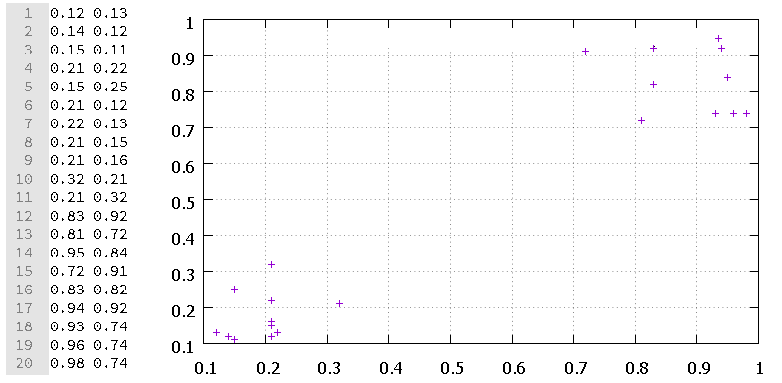
\includegraphics[scale=.9]{figures/simpleDataset.png}
	\caption{Two-dimensional dataset used in the initial experiment.}
	\label{fig:simpleDataset}
\end{figure*}


The initial experiment used the dataset presented on figure \ref{fig:simpleDataset} as input of the individuals (clustering algorithms). The configuration used for the GA to evolve the clustering algorithms is presented in table \ref{ga-configuration}. These values were set based on the work made by \cite{lourencco2012evolving}. Initially, the amount of generations was set to 600. But observing the evolution it was possible to realize that the GA was converging to the best solution approximately between the generations 80 and 130. Therefore it was decided to reduce the generations in order to save time.


\begin{table}[]
	\centering
	\caption{Configuration used in the GA}
	\label{ga-configuration}
	\begin{tabular}{|l|l|}
		\hline
		\textbf{Crossover  |  Probability}         & Single Point Crossover | 0.95     \\ \hline
		\textbf{Mutation | Probability}            & Integer Mutation          |  0.10 \\ \hline
		\textbf{Prune Operator | Probability}      & Prune Operator           | 0.05   \\ \hline
		\textbf{Duplication Operator | Probability} & Duplication Operator   | 0.05     \\ \hline
		\textbf{Population}                        & 100                               \\ \hline
		\textbf{Generations}                       & 200                               \\ \hline
	\end{tabular}
\end{table}


The GA proposed was executed 10 times and for comparison the k-means algorithm was also executed 10 times. Both results of GA (best individuals) and k-means (independent executions) were submitted to the same fitness function presented on \ref{equation:fitness}. Table \ref{tab:resultsInitial}
shows the average/standard deviation/min and max values of fitnesses obtained by the best individuals found by the GA in each run. Also the same statistics are presented for the k-means executions using the dataset presented on figure \ref{fig:simpleDataset}.
It is easy to see that GA in all executions was able to find an individual which is capable to obtain exactly the same fitness value that the k-means algorithm obtains. 


\begin{table}[]
	\centering
	\caption{Results of the initial experiment}
	\label{tab:resultsInitial}
	\begin{tabular}{|l|l|l|l|c|}
		\hline
		Algorithm                & Statistics & Fitness   & k                                             & \multicolumn{1}{l|}{Kruskal-Wallis Test} \\ \hline
		\multirow{4}{*}{GA}      & Average    & 0,8738090 & 2                                             & \multirow{8}{*}{False}                   \\ \cline{2-4}
		& Std Dev    & 0,0000000 & 0                                             &                                          \\ \cline{2-4}
		& Min        & 0,8738090 & 2                                             &                                          \\ \cline{2-4}
		& Max        & 0,8738090 & 2                                             &                                          \\ \cline{1-4}
		\multirow{4}{*}{K-Means} & Average    & 0,8738090 & \multicolumn{1}{c|}{\multirow{4}{*}{Fixed 2}} &                                          \\ \cline{2-3}
		& Std Dev    & 0,0000000 & \multicolumn{1}{c|}{}                         &                                          \\ \cline{2-3}
		& Min        & 0,8738090 & \multicolumn{1}{c|}{}                         &                                          \\ \cline{2-3}
		& Max        & 0,8738090 & \multicolumn{1}{c|}{}                         &                                          \\ \hline
	\end{tabular}
\end{table}

Since the initial experiment used a very simple and well separated database, a set of experiments were conducted using  four well-known clustering dataset points from UCI machine learning database \cite{uci}. Table \ref{uci-experiments} shows the amount of points (instances), how many attributes and the data type of the datasets. Below a more detailed description of the data used in the experiments is provided:

\begin{itemize}
	\item Pima Indians Diabetes: This database is from 768 patient females, with at least 21 years old, of Pima Indian heritage. The database has 8 attributes and is divided in two classes (0 negative or 1 positive for diabetes). The attribute summary are listed below:
	\begin{enumerate}
		\item Number of times pregnant.
		\item Plasma glucose concentration a 2 hours in an oral glucose tolerance test.
		\item  Diastolic blood pressure (mm Hg).
		\item  Triceps skin fold thickness (mm).
		\item  2-Hour serum insulin (mu U/ml).
		\item Body mass index $(weight in kg/(height in m)^2$).
		\item Diabetes pedigree function.
		\item Age (years).
	\end{enumerate}
	\item Statlog (Heart): This database is related to heart diseases. Obtained from 270 patients divided in two classes (1 - absence or 2 presence of heart disease). The attribute description is listed below:
	\begin{enumerate}
		\item Age.
		\item Sex.
		\item Chest pain type (4 values).
		\item Resting blood pressure.
		\item Serum cholesterol in mg/dl. 
		\item Fasting blood sugar $>$ 120 mg/dl.
		\item Resting electrocardiograph results (values 0,1,2).
		\item Maximum heart rate achieved.
		\item Exercise induced angina.
		\item Oldpeak = ST depression induced by exercise relative to rest.
		\item The slope of the peak exercise ST segment. 
		\item Number of major vessels (0-3) colored by flourosopy.
		\item thal: 3 = normal; 6 = fixed defect; 7 = reversible defect. 
	\end{enumerate}
	\item Iris: Probably the best known database for clustering techniques. It contains 3 classes of 50 instances each with 4 attributes. Each class refers to a type of iris plant. The attribute description is listed below:
	\begin{enumerate}
		\item Sepal length in cm.
		\item Sepal width in cm.
		\item Petal length in cm.
		\item Petal width in cm.
	\end{enumerate}
	
	\item Glass Identification: Database from glass type identification. This dataset has 7 classes and 10 attributes from 214 instances. The description for each attribute is listed below:
	\begin{enumerate}
		\item Id number: 1 to 214.
		\item RI: refractive index.
		\item Na: Sodium (unit measurement: weight percent in corresponding oxide, as are attributes 4-10).
		\item Mg: Magnesium.
		\item Al: Aluminum.
		\item Si: Silicon.
		\item K: Potassium.
		\item Ca: Calcium.
		\item Ba: Barium.
		\item Fe: Iron.
	\end{enumerate}
\end{itemize}


\begin{table}[]
	\centering
	\caption{UCI datasets used in the experiments}
	\label{uci-experiments}
	\begin{tabular}{|l|l|l|l|l}
		\cline{1-4}
		\textbf{Dataset Name} & \textbf{Instances} & \textbf{Attributes} & \textbf{Type}     &  \\ \cline{1-4}
		Pima Indians Diabetes & 768                & 8                   & Integer, Real     &  \\ \cline{1-4}
		Statlog (Heart)       & 270                & 13                  & Categorical, Real &  \\ \cline{1-4}
		Iris                  & 150                & 4                   & Real              &  \\ \cline{1-4}
		Glass Identification  & 214                & 10                  & Real              &  \\ \cline{1-4}
	\end{tabular}
\end{table}


As before, in the initial experiment, the GA was executed 10 independent runs with each dataset using the same configuration presented in table \ref{tab:resultsInitial}. The evaluation of the individuals was made using the fitness function presented on equation \ref{equation:fitness}.
The results were summarized by means of average, standard deviation, minimum and maximum values of the fitness value,  from the best individual of each run of the GA. The amount of clusters (k) found are also presented.
In order to make comparisons, the k-means algorithm was executed 10 times with different k values. The k value for k-means was varied within the range 2 to 7 and only the best k configuration (the one whose obtained the highest fitness values) will be presented. Table \ref{results-ga-and-kmeans} shows the results described above. 


\begin{table*}[]
	\centering
	\caption{Results of GA best individual and also the fitness obtained by k-means algorithm}
	\label{results-ga-and-kmeans}
	\begin{tabular}{|c|c|c|c|c|c|}
		\hline
		\textbf{Dataset}                       & \textbf{Algorithm}       & \textbf{Statistics} & \textbf{Fitness} & \textbf{k}               & Kruskal-Wallis Test   \\ \hline
		\multirow{8}{*}{Pima Indians Diabetes} & \multirow{4}{*}{GA}      & Average             &                  &                          & \multirow{8}{*}{}     \\ \cline{3-5}
		&                          & Std Dev             &                  &                          &                       \\ \cline{3-5}
		&                          & Min                 &                  &                          &                       \\ \cline{3-5}
		&                          & Max                 &                  &                          &                       \\ \cline{2-5}
		& \multirow{4}{*}{K-Means} & Average             &                  &                          &                       \\ \cline{3-5}
		&                          & Std Dev             &                  &                          &                       \\ \cline{3-5}
		&                          & Min                 &                  &                          &                       \\ \cline{3-5}
		&                          & Max                 &                  &                          &                       \\ \hline
		\multirow{8}{*}{Statlog (Heart)}       & \multirow{4}{*}{GA}      & Average             & 0.410924         & 2                        & \multirow{8}{*}{TRUE} \\ \cline{3-5}
		&                          & Std Dev             & 0.019960         & 0                        &                       \\ \cline{3-5}
		&                          & Min                 & 0.381797         & 2                        &                       \\ \cline{3-5}
		&                          & Max                 & 0.44972          & 2                        &                       \\ \cline{2-5}
		& \multirow{4}{*}{K-Means} & Average             & 0.383325         & \multirow{4}{*}{Fixed 2} &                       \\ \cline{3-4}
		&                          & Std Dev             & 0.001523         &                          &                       \\ \cline{3-4}
		&                          & Min                 & 0.382144         &                          &                       \\ \cline{3-4}
		&                          & Max                 & 0.385095         &                          &                       \\ \hline
		\multirow{8}{*}{Glass Identification}  & \multirow{4}{*}{GA}      & Average             & 0.602340         & 2                        & \multirow{8}{*}{TRUE} \\ \cline{3-5}
		&                          & Std Dev             & 0.005321         & 0                        &                       \\ \cline{3-5}
		&                          & Min                 & 0.593869         & 2                        &                       \\ \cline{3-5}
		&                          & Max                 & 0.610906         & 2                        &                       \\ \cline{2-5}
		& \multirow{4}{*}{K-Means} & Average             & 0.624821         & \multirow{4}{*}{Fixed 2} &                       \\ \cline{3-4}
		&                          & Std Dev             & 0.000007         &                          &                       \\ \cline{3-4}
		&                          & Min                 & 0.624818         &                          &                       \\ \cline{3-4}
		&                          & Max                 & 0,624836         &                          &                       \\ \hline
		\multirow{8}{*}{Iris}                  & \multirow{4}{*}{GA}      & Average             & 0.6442809        & 2                        & \multirow{8}{*}{TRUE} \\ \cline{3-5}
		&                          & Std Dev             & 0.0135472        & 0                        &                       \\ \cline{3-5}
		&                          & Min                 & 0.6244826        & 2                        &                       \\ \cline{3-5}
		&                          & Max                 & 0.6679046        & 2                        &                       \\ \cline{2-5}
		& \multirow{4}{*}{K-Means} & Average             & 0.6813042        & \multirow{4}{*}{Fixed 2} &                       \\ \cline{3-4}
		&                          & Std Dev             & 0,0000000        &                          &                       \\ \cline{3-4}
		&                          & Min                 & 0,6813042        &                          &                       \\ \cline{3-4}
		&                          & Max                 & 0,6813043        &                          &                       \\ \hline
	\end{tabular}
\end{table*}



\begin{table*}[]
	\centering
	\caption{Statistic of execution time of the algorithms}
	\label{resultsTimeExecution}
	\begin{tabular}{|c|c|c|c|c|}
		\hline
		\textbf{Dataset}                       & \multicolumn{1}{l|}{\textbf{Statistics}} & \multicolumn{1}{l|}{\textbf{\begin{tabular}[c]{@{}l@{}}GA Execution\\ Time (h)\end{tabular}}} & \multicolumn{1}{l|}{\textbf{\begin{tabular}[c]{@{}l@{}}GA Best Individual \\ Execution Time (ms)\end{tabular}}} & \multicolumn{1}{l|}{\textbf{\begin{tabular}[c]{@{}l@{}}K-Means\\ Execution Time (ms)\end{tabular}}} \\ \hline
		\multirow{4}{*}{Pima Indians Diabetes} & Average                                  & \multicolumn{1}{l|}{}                                                                         & \multicolumn{1}{l|}{}                                                                                           & \multicolumn{1}{l|}{}                                                                               \\ \cline{2-5} 
		& Std Dev                                  & \multicolumn{1}{l|}{\textbf{}}                                                                & \multicolumn{1}{l|}{\textbf{}}                                                                                  & \multicolumn{1}{l|}{\textbf{}}                                                                      \\ \cline{2-5} 
		& Min                                      & \multicolumn{1}{l|}{\textbf{}}                                                                & \multicolumn{1}{l|}{\textbf{}}                                                                                  & \multicolumn{1}{l|}{\textbf{}}                                                                      \\ \cline{2-5} 
		& Max                                      & \multicolumn{1}{l|}{\textbf{}}                                                                & \multicolumn{1}{l|}{\textbf{}}                                                                                  & \multicolumn{1}{l|}{\textbf{}}                                                                      \\ \hline
		\multirow{4}{*}{Statlog (Heart)}       & Average                                  & 38.6                                                                                          & 1468.8                                                                                                          & 20.3                                                                                                \\ \cline{2-5} 
		& Std Dev                                  & 11.1                                                                                          & 243.5                                                                                                           & 11.6                                                                                                \\ \cline{2-5} 
		& Min                                      & 23.0                                                                                          & 885.0                                                                                                           & 7.0                                                                                                 \\ \cline{2-5} 
		& Max                                      & 56.0                                                                                          & 1738.0                                                                                                          & 52.0                                                                                                \\ \hline
		\multirow{4}{*}{Glass Identification}  & Average                                  & 19.6                                                                                          & 2602.1                                                                                                          & 14.8                                                                                                \\ \cline{2-5} 
		& Std Dev                                  & 2.1                                                                                           & 502.69                                                                                                          & 13.0                                                                                                \\ \cline{2-5} 
		& Min                                      & 15.0                                                                                          & 1610.0                                                                                                          & 3.0                                                                                                 \\ \cline{2-5} 
		& Max                                      & 22.0                                                                                          & 3185.0                                                                                                          & 45.0                                                                                                \\ \hline
		\multirow{4}{*}{Iris}                  & Average                                  & 8.5                                                                                           & 1074.5                                                                                                          & 15.1                                                                                                \\ \cline{2-5} 
		& Std Dev                                  & 2.7                                                                                           & 383.9                                                                                                           & 14.9                                                                                                \\ \cline{2-5} 
		& Min                                      & 4.5                                                                                           & 558.0                                                                                                           & 7.0                                                                                                 \\ \cline{2-5} 
		& Max                                      & 12.0                                                                                          & 1786.0                                                                                                          & 59.0                                                                                                \\ \hline
	\end{tabular}
\end{table*}


Looking to table \ref{results-ga-and-kmeans} it is possible to see that for the Pima Indian Diabetes, our approach reached BLAH average of the fitness values obtained by the bests individuals of 10 executions. While the k-means algorithm obtained a lesser value BLAH on 10 executions. 
In the case of the Statlog (Heart) database the GA obtained a better average value of 0.410 while k-means algorithm reached 0.383 with statistic difference according with the Kruskal and Wallis test.
In the Glass database the GA obtained a lesser value than k-means, 0.603 and 0.624 respectively also with statistic difference according to Kruskal and Wallis test. 
Finally for the Glass database the best individuals of GA obtained 0.644 and the k-means reached 0.681, again with statistic difference according to Kruskal and Wallis test.
Also it is possible to note that for all 10 executions of the GA the generated algorithms decided to divide in two clusters the input data from the databases. In the case of the k-means algorithm the results that presented the highest fitness values were also using $k=2$. For the sake of space the results with $k = (3,4,5,6,7)$ were suppressed.

Table \ref{resultsTimeExecution} presents some time information of the algorithms. The statistic summary of 10 GA executions, in hours, is presented in the third column. In the fourth column shows the statistics summary of time taken, in milliseconds, to execute 10 times the best individual found by the GA. The fifth columns presents the statistics summary to execute 10 times the k-means algorithm.

Another set of experiments were conducted to evaluate the research question (Q2). This experiments were design to evaluate if the generated algorithms are able to generalize well across unknown databases. Hence the best individual found for each database were selected and executed 10 times against the other databases (the ones that were not used in the GA to find the respective generated algorithm). The results are separated by dataset. Tables \ref{results:generalizationIris},\ref{results:generalizationGlass},\ref{results:generalizationHeart} shows the results for iris, heart, glass and diabetes respectively.

\begin{table}[]
	\centering
	\caption{Results obtained using the best algorithms found on glass, heart and diabetes applied in the iris dataset}
	\label{results:generalizationIris}
	\begin{tabular}{|c|l|l|l|l|l|}
		\hline
		\textbf{Dataset}       & \multicolumn{1}{c|}{\textbf{\begin{tabular}[c]{@{}c@{}}Individual\\ Algorithm\end{tabular}}} & \multicolumn{1}{c|}{\textbf{Statistics}} & \multicolumn{1}{c|}{\textbf{Fitness}} & \multicolumn{1}{c|}{\textbf{k}} & \multicolumn{1}{c|}{\textbf{Time}} \\ \hline
		\multirow{12}{*}{Iris} & \multirow{4}{*}{\begin{tabular}[c]{@{}l@{}}Best Found\\ on Glass\end{tabular}}               & Average                                  & 0.5980934                              & 2                               & \multirow{4}{*}{2 (seconds)}       \\ \cline{3-5}
		&                                                                                              & Std Dev                                  & 0,1051669                          & 0                               &                                    \\ \cline{3-5}
		&                                                                                              & Min                                      & 0,3942573                           & 2                               &                                    \\ \cline{3-5}
		&                                                                                              & Max                                      & 0,6869726                             & 2                               &                                    \\ \cline{2-6} 
		& \multirow{4}{*}{\begin{tabular}[c]{@{}l@{}}Best Found \\ on Heart\end{tabular}}              & Average                                  & 0,4373911                           & 2                               & \multirow{4}{*}{2 (seconds)}       \\ \cline{3-5}
		&                                                                                              & Std Dev                                  & 0,2083442                           & 0                               &                                    \\ \cline{3-5}
		&                                                                                              & Min                                      & 0,1328811                           & 2                               &                                    \\ \cline{3-5}
		&                                                                                              & Max                                      & 0,6641139                             & 2                               &                                    \\ \cline{2-6} 
		& \multirow{4}{*}{\begin{tabular}[c]{@{}l@{}}Best Found \\ on Diabetes\end{tabular}}           & Average                                  &                                       &                                 &                                    \\ \cline{3-6} 
		&                                                                                              & Std Dev                                  &                                       &                                 &                                    \\ \cline{3-6} 
		&                                                                                              & Min                                      &                                       &                                 &                                    \\ \cline{3-6} 
		&                                                                                              & Max                                      &                                       &                                 &                                    \\ \hline
	\end{tabular}
\end{table}

Analyzing table \ref{results:generalizationIris} we can see that the best individual found using the heart dataset reached a fitness average of 0.437 and the best found using glass data set was able to reach an average of 0.598. Comparing with fitness average found by the best individuals found by GA using iris dataset which reached 0.644 (table \ref{results-ga-and-kmeans}). It is possible to see that best algorithms found using the other datasets did not perform so well when applied to iris dataset.

Looking to table \ref{results:generalizationGlass}, as before, the best algorithms found using iris, heart and diabetes datasets also did not perform well when applied to glass dataset. It was obtained an average of 0.554 (best from iris) and 0.520 (best from heart) while the best found using the glass dataset obtained 0.602 and the k-means 0.624.

Table \ref{results:generalizationHeart} shows the same behavior, when applying the best algorithms found by iris, glass an diabetes datasets on heart dataset. The results found by those were 0.277 (best from iris) and 0.306 (best from glass), very low in relation to 0.410 and 0.383 from the best found using the heart dataset and the k-means algorithm respectively.


\begin{table}[]
	\centering
	\caption{Results obtained using the best algorithms found on iris, heart and diabetes applied in the glass dataset}
	\label{results:generalizationGlass}
	\begin{tabular}{|c|l|l|l|l|l|}
		\hline
		\textbf{Dataset}        & \multicolumn{1}{c|}{\textbf{\begin{tabular}[c]{@{}c@{}}Individual\\ Algorithm\end{tabular}}} & \multicolumn{1}{c|}{\textbf{Statistics}} & \multicolumn{1}{c|}{\textbf{Fitness}} & \multicolumn{1}{c|}{\textbf{k}} & \multicolumn{1}{c|}{\textbf{Time}} \\ \hline
		\multirow{12}{*}{Glass} & \multirow{4}{*}{\begin{tabular}[c]{@{}l@{}}Best Found\\ on Iris\end{tabular}}                & Average                                  & 0.554890                          & 2                               & \multirow{4}{*}{3 (seconds)}       \\ \cline{3-5}
		&                                                                                              & Std Dev                                  & 0.055117                              & 0                               &                                    \\ \cline{3-5}
		&                                                                                              & Min                                      & 0.462729                              & 2                               &                                    \\ \cline{3-5}
		&                                                                                              & Max                                      & 0.621245                              & 2                               &                                    \\ \cline{2-6} 
		& \multirow{4}{*}{\begin{tabular}[c]{@{}l@{}}Best Found \\ on Heart\end{tabular}}              & Average                                  & 0.520432                              & 2                               & \multirow{4}{*}{4 (seconds)}       \\ \cline{3-5}
		&                                                                                              & Std Dev                                  & 0.070336                              & 0                               &                                    \\ \cline{3-5}
		&                                                                                              & Min                                      & 0.354634                              & 2                               &                                    \\ \cline{3-5}
		&                                                                                              & Max                                      & 0.607885                              & 2                               &                                    \\ \cline{2-6} 
		& \multirow{4}{*}{\begin{tabular}[c]{@{}l@{}}Best Found \\ on Diabetes\end{tabular}}           & Average                                  &                                       &                                 &                                    \\ \cline{3-6} 
		&                                                                                              & Std Dev                                  &                                       &                                 &                                    \\ \cline{3-6} 
		&                                                                                              & Min                                      &                                       &                                 &                                    \\ \cline{3-6} 
		&                                                                                              & Max                                      &                                       &                                 &                                    \\ \hline
	\end{tabular}
\end{table}



\begin{table}[]
	\centering
	\caption{Results obtained using the best algorithms found on iris, glass and diabetes applied in the heart dataset}
	\label{results:generalizationHeart}
	\begin{tabular}{|c|l|l|l|l|l|}
		\hline
		\textbf{Dataset}        & \multicolumn{1}{c|}{\textbf{\begin{tabular}[c]{@{}c@{}}Individual\\ Algorithm\end{tabular}}} & \multicolumn{1}{c|}{\textbf{Statistics}} & \multicolumn{1}{c|}{\textbf{Fitness}} & \multicolumn{1}{c|}{\textbf{k}} & \multicolumn{1}{c|}{\textbf{Time}} \\ \hline
		\multirow{12}{*}{Heart} & \multirow{4}{*}{\begin{tabular}[c]{@{}l@{}}Best Found\\ on Iris\end{tabular}}                & Average                                  & 0,2777372                             & 2                               & \multirow{4}{*}{17 (seconds)}      \\ \cline{3-5}
		&                                                                                              & Std Dev                                  & 0,1036269                             & 0                               &                                    \\ \cline{3-5}
		&                                                                                              & Min                                      & 0,0835615                             & 2                               &                                    \\ \cline{3-5}
		&                                                                                              & Max                                      & 0,3860393                             & 2                               &                                    \\ \cline{2-6} 
		& \multirow{4}{*}{\begin{tabular}[c]{@{}l@{}}Best Found \\ on Glass\end{tabular}}              & Average                                  & 0,3062312                             & 2                               & \multirow{4}{*}{18 (seconds)}      \\ \cline{3-5}
		&                                                                                              & Std Dev                                  & 0,1148123                             & 0                               &                                    \\ \cline{3-5}
		&                                                                                              & Min                                      & 0,1154442                             & 2                               &                                    \\ \cline{3-5}
		&                                                                                              & Max                                      & 0,5377623                       & 2                               &                                    \\ \cline{2-6} 
		& \multirow{4}{*}{\begin{tabular}[c]{@{}l@{}}Best Found \\ on Diabetes\end{tabular}}           & Average                                  &                                       &                                 &                                    \\ \cline{3-6} 
		&                                                                                              & Std Dev                                  &                                       &                                 &                                    \\ \cline{3-6} 
		&                                                                                              & Min                                      &                                       &                                 &                                    \\ \cline{3-6} 
		&                                                                                              & Max                                      &                                       &                                 &                                    \\ \hline
	\end{tabular}
\end{table}



\section{Discussion}

After the experiments conducted it was possible to answer both research questions described in section \ref{sec:research-questions}.
\begin{itemize}
	\item Q1 - Based on the experiments conducted is was possible to check that the generated algorithms are able to reach good and acceptable values for our fitness function (which is based on the silhouette index). The fitness values obtained by the generated algorithms in two of four experiments were higher than the ones obtained by the k-means algorithm. The difference between the fitness values obtained by k-means and the approach proposed here is very small. Our conclusion was that in this context the generated algorithms proved to be competitive with k-means algorithm. It is possible to highlight one convenience of the proposed approach: there is no need to configure a k value which usually is a non-trivial task as mentioned by many authors \cite{pham2005selection, yan2005methods, tibshirani2001estimating}.
	\item Q2 - From the experiments executed to evaluate the ability of generalization of the generated algorithms it was possible to check that they do not generalize well when facing an unknown dataset (that was not used to find the algorithm). In all cases the generated algorithms obtained low values of fitness in other datasets. Thus the conclusion is that in this context the generated algorithms are not able to generalize well using other datasets. It is due to the over-specialization of the algorithms within the dataset used to find it.
\end{itemize}

\section{Conclusion}

Grammatical evolution is a form of genetic programming which uses a grammar to map between the genotype and the phenotype. The definition of a good terminal set is crucial for the success of an GE approach. In this work it was defined a grammar and a terminal and function sets in order to evolve a population of clustering algorithms through a GA. To evaluate the generated algorithms: a fitness function based on the silhouette index was designed. A set of experiments were conducted and compared with the k-means algorithm. The initial experiment conducted was very simple, however it was useful to check if the proposed approach had potential. In the first experiment the best individual, found by the grammatical evolution approach, was able to reach exactly the same fitness values compared to k-means in 10 independent executions. After the initial experiment a set of experiments using some of the UCI classification databases were conducted. In 2 of 4 experiments the proposed approach reached higher values when compared with the k-means algorithm. Based on the conducted experiments it was possible to conclude that the proposed approach can generated good clustering algorithms competitive with the k-means algorithm.


\section{Threats to validity}

Some threats to validity are discussed in this section:
\begin{itemize}
	\item The parameters configuration was not tuned: Due to time constraints the grammatical evolution process was not tuned. The configuration was selected mainly based on literature values and some empirical choices. It is possible that using a tuned configuration the results get improvements.
	\item The experiments were conducted using only 4 datasets: It is necessary to execute more experiments with a broader range of datasets in order to evaluate if the same behavior is maintained.
\end{itemize}

%Referências
\bibliographystyle{plain}
\bibliography{references}

% that's all folks
\end{document}